% !TeX program = xelatex
% Compile with XeLaTeX. Edit each response directly below the quoted comment.
% Comments are transcribed from the current Word files. Replies are from the current response PDFs.
\documentclass[12pt,a4paper]{article}
\usepackage[top=25.4mm,bottom=25.4mm,left=31.75mm,right=31.75mm]{geometry}
\usepackage{fontspec}
\usepackage{amsmath}
\usepackage{xcolor}
\usepackage{graphicx}
\setmainfont{Times New Roman}
\setlength{\parindent}{0pt}
\setlength{\parskip}{6pt}
\setlength{\emergencystretch}{1.5em}

\begin{document}

\begin{center}
  {\Large\bfseries Response to Reviewers}
\end{center}

\section*{Reviewer 1}

This manuscript investigates adaptive event-triggered control for interval type-2 (IT-2) fuzzy cyber-physical systems subject to stochastic deception attacks and Markov-type actuator failures. The combination of adaptive transmission and membership-function-derivative-dependent regional control is relevant to secure networked control. The numerical examples provide an initial illustration of the proposed framework. After reading, the primary features and contributions of this article are sound compared to some existing publications. However, the following aspects should be seriously considered to improve the presentation quality of this investigation.

\subsection*{R1.1}

\textbf{Comment.}
\begin{quote}
\raggedright
It is noted that your manuscript needs careful editing, such as the English grammar and sentence structure so that the goals and results in your work are friendly to the weak in English.
\end{quote}

\textbf{Response.}
Thank you for this suggestion. We have revised the Abstract, Introduction, problem formulation, explanatory text in Section 3, numerical discussion, and Conclusion. The Abstract now proceeds from the attack/failure setting to the adaptive transmission and regional design, then to the sufficient conditions and numerical illustrations. We have corrected subject–verb agreement, removed a duplicated full stop and an unnecessary comma, clarified transitions, and made the terminology and abbreviations more consistent. In particular, the controller-gain description now refers to the gain for an individual fuzzy rule, and the distinction between an initial state in Example 2 and that of Example 1 is explicit. The detailed companion document records every implemented replacement, including punctuation and whitespace, rather than providing only selected examples. These changes improve exposition without modifying the displayed mathematical conditions or the numerical data.


\textbf{Revision location.} Clean manuscript pp. 1–5, 7, 10–11, 13–14, 17–18. Marked manuscript pp. 1–8, 11–12, 14–15, 18–20. Revision items M01, M02, M03, M04, M05, M06, M09, M10, M11, M12, M13, M14, M16, M19, M20, M21, M22, M27, M28, M29, M30, M31, M34, M37, M38, M47, M53, M54, M56, M57, M58.

\subsection*{R1.2}

\textbf{Comment.}
\begin{quote}
\raggedright
\textcolor{red}{The} motivation for jointly considering deception attacks, actuator failures, and communication limitations needs clarification. Could the authors clarify why these factors require simultaneous consideration and how their combined effects influence closed-loop stability and $\mathrm{H}_{\infty}$ performance? \textcolor{red}{Complete}
\end{quote}

\textbf{Response.}
Thank you for this comment. In Eq.~(15), the actuator scales a command based on the most recently released sample. If that sample was falsified, the feedback may continue to use incorrect data while an actuator fault reduces the effectiveness of the command. This can impair the controller's ability both to drive the state back to equilibrium and to attenuate external disturbances. The two revised sentences are quoted below.\\

\textcolor{red}{With event-triggered transmission, the controller may continue to use a falsified sample until the next release, while an actuator fault may weaken the command computed from that sample. These effects must therefore be considered together when assessing whether the feedback can stabilize the plant and achieve the prescribed $\mathrm{H}_\infty$ disturbance attenuation.} (The fifth paragraph in the introduction)

% Previous editable template draft and location notes.
% Thank you for this comment. We have added a paragraph following the actuator-failure discussion in the Introduction. It explains that deception attacks alter the information supplied to the controller, actuator failures alter the effectiveness of the input delivered to the plant, and event-triggered transmission retains the last transmitted sample between releases. The resulting sampling error, corrupted feedback, and actuator effectiveness enter the same closed-loop dynamics. Their coexistence therefore motivates evaluating stability and disturbance attenuation jointly under the specified models. This explanation identifies the coupling relevant to the control problem without suggesting that separate studies of the individual mechanisms are uninformative.
%
%
% \textbf{Revision location.} Clean manuscript p. 2. Marked manuscript p. 2. Revision items M07.

\subsection*{R1.3}

\textbf{Comment.}
\begin{quote}
\raggedright
The author should check the References carefully throughout this paper, there are many references which not fit our style need some modification and there is something wrong with the formatting of the Reference.
\end{quote}

\textbf{Response.}
% Earlier question, draft response, and revision location (retained for reference).
% The Introduction cites several recent publications, but the relationship between the closest studies and the present contribution could be explained more explicitly. Please connect recent work on event-triggered control of IT-2 fuzzy systems, secure control under deception attacks, and actuator-failure compensation. Could the authors further clarify the methodological differences between the proposed approach and the most closely related studies?
% \textbf{Response.}
% Thank you for this comment. We have expanded the comparison immediately before the contribution list. Two directly relevant studies have been added: Liu, Ling, and Zhang (2025), on torus-event-based sliding-mode control of discrete-time IT-2 fuzzy systems under deception attacks, and Chandrasekar et al. (2026), on adaptive event-triggered asynchronous control of uncertain IT-2 fuzzy Markov jump systems with deception attacks. Their publication details and the methodological descriptions were checked against the publishers’ article pages. The comparison also explicitly cites the existing work by Chen et al. (2023) on probabilistic event-triggered control under cyberattacks and actuator failures. We distinguish the present continuous-time formulation, Markov-type actuator effectiveness, and derivative-sign-based regional synthesis. We also state that joint attack/failure modeling and adaptive event triggering are not, by themselves, claimed as new. The additions therefore strengthen positioning through concrete connections and distinctions, rather than citation count alone.
%
%
% \textbf{Revision location.} Clean manuscript p. 2. Marked manuscript p. 2. Revision items M08.

\subsection*{R1.4}

\textbf{Comment.}
\begin{quote}
\raggedright
\textcolor{red}{Please} clarify the physical meaning of the actuator-failure parameters $F_{i0}$, $F_{i1}$ and the Markov transition-rate matrix used in the simulation. How are the failure-level bounds and the transition rates chosen, and does the closed-loop system remain stable under more severe failure modes? \textcolor{red}{Complete}
\end{quote}

\textbf{Response.}
Thank you for this comment.\\

1) In Eq.~(13), $F_{i0}$ and $F_{i1}$ denote the midpoint and half-width, respectively, of the actuator effectiveness interval in mode $i$. For the simulation in Example~1, we chose $[0.8,1]$ and $[0.6,1]$ to represent two degrees of partial actuator failure. At the lower bounds, the actuator delivers $80\%$ of the commanded input in mode~1 and $60\%$ in mode~2.\\

2) We used illustrative transition rates of $\lambda_{12}=0.6$ and $\lambda_{21}=1.2$ per unit time to model switching between the two failure modes. With these values, the mean residence time in the more degraded mode is half that in the less degraded mode.\\

3) Under the conditions of Theorem~3.3, the controller designed in Example~1 guarantees closed-loop stability as the actuator switches between the two specified failure modes. This guarantee includes the more severe case in mode~2, where the actuator can deliver as little as $60\%$ of the commanded input. For a wider failure interval, the same controller retains this guarantee provided that the stability conditions hold over the enlarged interval with its gains fixed.

% Previous editable template draft and location notes.
% % Earlier question, draft response, and revision location (retained for reference).
% % Remark 2.2 identifies the equilibrium value of the adaptive threshold, but its practical interpretation could be clearer. How do the adaptive threshold dynamics interact with the triggering condition and state error, particularly under different initial conditions?
% % \textbf{Response.}
% % Thank you for this suggestion. We have revised the sentence following the adaptive law and expanded Remark 2.2. The text now identifies 1/\(\sigma\) as the equilibrium threshold and distinguishes the two possible adjustment directions: with a positive threshold and nonzero error, the threshold increases below 1/\(\sigma\) and decreases above it. Its derivative is zero at equilibrium or when the triggering error is zero. We therefore do not assume that the threshold increases, or decreases, for every initial condition. We also explain that a larger threshold makes the triggering inequality harder to satisfy when the sampled state, error, and weighting matrix are held fixed. Actual release times still depend on their joint evolution. The triggering inequality and adaptive differential equation are unchanged.
% %
% %
% % \textbf{Revision location.} Clean manuscript p. 4. Marked manuscript p. 5. Revision items M17, M18.

\subsection*{R1.5}

\textbf{Comment.}
\begin{quote}
\raggedright
\textcolor{red}{The} operational regions are determined by the signs of the membership-function derivatives. For readers unfamiliar with this construction, the link between a derivative sign pattern and the associated matrix constraints may not be immediately apparent. Could the authors explain how the signs of the membership-function derivatives determine the regional constraints and how these constraints are incorporated into controller synthesis? \textcolor{red}{Complete}
\end{quote}

\textbf{Response.}
\begingroup
\setlength{\parskip}{6pt}
\noindent Thank you for raising this point. The two-rule system in Example~1 illustrates how the derivative sign determines a regional constraint. Since $h_1+h_2=1$, we have $\dot P_{ih}=\dot h_1(P_{i1}-P_{i2})$. To ensure $\dot P_{ih}\preceq 0$, we impose $P_{i1}-P_{i2}\succeq 0$ when $\dot h_1\leq 0$ and $P_{i1}-P_{i2}\preceq 0$ when $\dot h_1>0$. Applying the same reasoning to the other matrix derivatives, according to their required signs, gives the two constraint sets $\mathcal C_1$ and $\mathcal C_2$. We then solve the LMIs of Theorem~3.3 under the corresponding constraint set to obtain the controller gains and triggering weight matrix for each region.\par
\noindent \textbf{Remark 2.4.} Lemma 2.1 indicates that the state space can be partitioned into $2^{r-1}$ operational regions, denoted by $\mathcal{V}_l$ ($l = 1,2,\dots,2^{r-1}$), according to the sign combinations of $\dot{h}_v$. \textcolor{red}{Taking rule $r$ as the reference, Eq.~(16) ensures that each term $\dot h_v(G_v-G_r)$ is negative semidefinite by requiring $G_v-G_r\succeq 0$ when $\dot h_v\leq 0$ and $G_v-G_r\preceq 0$ when $\dot h_v>0$. For each region $\mathcal V_l$, the inequalities obtained according to the required sign of each matrix derivative form the constraint set $\mathcal C_l$. We impose $\mathcal C_l$ when solving the LMIs of Theorem~3.3 to obtain the controller gains $K_n^l$ and the triggering weight matrix $S^l$ for that region.} (Remark 2.4)\par
\endgroup

\subsection*{R1.6}

\textbf{Comment.}
\begin{quote}
\raggedright
\textcolor{red}{Table} 1 reports packet counts and saving rates for several values of $\sigma$, but the implications of the trend could be discussed more explicitly. The reported packet count increases from 85 to 164 as $\sigma$ rises from 4 to 20, while the saving rate decreases from 78.75\% to 59.00\%. Could the authors explain why the packet count increases and the saving rate decreases as $\sigma$ rises, and how this trend relates to the adaptive threshold and triggering condition under the tested settings? \textcolor{red}{Complete}
\end{quote}

\begingroup
\setlength{\parskip}{6pt}
\textbf{Response.}
Thank you for this suggestion. Equation~(6) shows that a larger $\sigma$ lowers the equilibrium threshold $1/\sigma$. A lower threshold in (5) means that a smaller change from the last transmitted sample can trigger a new transmission. In Table~1, the number of packets transmitted over the same 400 sampling instants rose from 85 to 164, so the saving rate fell from $78.75\%$ to $59.00\%$. We have added this explanation to the paragraph introducing Table~1.\par
\noindent Table~1 compares the proposed AETM with the time-triggered mechanism, which transmits all 400 samples. \textcolor{red}{Increasing $\sigma$ from 4 to 20 lowers the equilibrium value $1/\sigma$ of the adaptive threshold from 0.25 to 0.05. For a given sampled state and weighting matrix, a lower threshold $\delta(t)$ allows a smaller sampling error to trigger transmission under (5). This is consistent with the higher packet counts and lower saving rates observed in Table~1.} (The paragraph introducing Table~1 in Example~1)\par
\endgroup
% Previous working draft for this comment.
% \textbf{Response.}
% Thank you for this suggestion. We have expanded the discussion after Table 1 and stated the time-triggered baseline of 400 candidate transmissions. The saving rate is defined as the fraction of baseline transmissions avoided. The text connects the reported increase from 85 to 164 packets, and decrease from 78.75\% to 59.00\%, to the decrease of the equilibrium threshold from 0.25 to 0.05 as \(\sigma\) increases from 4 to 20. For fixed sampled state, error, and weighting matrix, a smaller threshold makes the triggering condition easier to satisfy. We explicitly qualify this interpretation: the actual count also depends on the closed-loop trajectory, threshold dynamics, and resulting design matrices. Thus, the table documents the observed communication trade-off for these settings and is not presented as a universal monotonicity result. The entries in Table 1 have not been altered.
% \textbf{Revision location.} Clean manuscript p. 16. Marked manuscript p. 17. Revision items M45, M46.

\subsection*{R1.7}

\textbf{Comment.}
\begin{quote}
\raggedright
\textcolor{red}{The} parameters $\xi_1$, $\xi_2$, and $\tau$ introduced in Theorems 3.2 and 3.3 are not explained. Please clarify their role in the LMI transformation, how they are chosen in the simulation, and whether the feasibility of the conditions is sensitive to their values. \textcolor{red}{Complete}
\end{quote}

\begingroup
\setlength{\parskip}{6pt}
\textbf{Response.}
Thank you for asking how these parameters enter the design and how their values are chosen. The scalars $\xi_1$ and $\xi_2$ fix the proportions among the slack matrices in Theorem~3.2. In Theorem~3.3, $\tau$ sets the relative weights of the two terms used to bound the actuator uncertainty. We prescribe the three scalars before solving the LMIs and use feasibility in both regions as the selection criterion. The nominal choices $(0.01,0.01,0.8)$ in Example~1 and $(2,4,2)$ in Example~2 both admit a solution in each region at $h=0.05$ and $\gamma=2$. We also checked sensitivity by re-solving the two regional problems after changing one scalar at a time by $-10\%$ or $+10\%$. All 24 perturbed regional problems were feasible. We have added the parameter interpretation to Remark~3.2 and the sensitivity results to the opening paragraph of Section~4.\par
\noindent \textbf{Remark 3.2.} \textcolor{red}{In Theorem~3.2, the relations $Q_2=\xi_1Q_1$ and $Q_3=\xi_2Q_1$ allow a common change of variables under which the gains enter the LMIs linearly through $\widetilde K_n=K_nQ_1^{-1}$.} In Theorem~3.3, the scaling parameter $\tau > 0$ is introduced to handle the norm-bounded uncertainty matrix $V_i$ resulting from stochastic actuator failures. \textcolor{red}{Young's inequality bounds the resulting cross term by two quadratic terms, with weight $\tau$ on the term involving $B_mF_{i1}$ and weight $1/\tau$ on the term involving $\widetilde K_n$.} (Remark~3.2)\par
\noindent This section considers an engineering-motivated example and a numerical simulation study to assess the effectiveness and applicability of the developed control scheme. \textcolor{red}{In each example, we prescribe $(\xi_1,\xi_2,\tau)$ and check that the LMIs of Theorem~3.3 are feasible separately under $\mathcal C_1$ and $\mathcal C_2$ at $h=0.05$ and $\gamma=2$. To assess sensitivity, we increased and decreased each scalar by $10\%$ in turn, holding the other two at their reported values. Both regional LMI problems remained feasible at all six perturbed settings in each example.} (The opening paragraph of Section~4)\par
\endgroup
% Earlier question, draft response, and revision location (retained for reference).
% The manuscript derives sufficient conditions for stability and \(H_\infty\) performance in terms of LMIs. The relationship between these two objectives could be explained more explicitly after the theorem statement. A brief interpretation would help readers distinguish the stability requirement from the disturbance-attenuation requirement..
% \textbf{Response.}
% Thank you for this comment. We have added an explanatory paragraph immediately after Theorem 3.1 and its proof, before Remark 3.1. It maps the two objectives to Definition 2.1: stability concerns the unforced closed loop, whereas the prescribed \(H_\infty\) level concerns the expected output-energy bound relative to disturbance energy for square-integrable disturbances under the definition’s zero-initial-condition convention. It identifies the output matrix C and performance parameter \(\gamma\) as the terms encoding the output–disturbance requirement in the same sufficient-condition framework. The paragraph also notes that infeasibility of these sufficient LMIs does not, by itself, establish instability. This is an interpretation of the stated result; the theorem conditions and derivation are retained.
%
%
% \textbf{Revision location.} Clean manuscript p. 11. Marked manuscript p. 11. Revision items M32.

\subsection*{R1.8}

\textbf{Comment.}
\begin{quote}
\raggedright
\textcolor{red}{There} are several minor numerical and grammatical errors that should be corrected. First, the communication saving rate in Example 2 should be 83.75\% rather than 83.79\%. Second, in the proof of Theorem 3.1, ``condition (22) guarantee'' should read ``condition (22) guarantees''. Please check the manuscript for similar issues elsewhere. \textcolor{red}{Complete}
\end{quote}

\begingroup
\setlength{\parskip}{3pt}
\textbf{Response.}
Thank you for pointing out these errors.\par
\noindent 1) In Example~2, 65 transmissions occurred over 400 candidate sampling instants, giving a saving rate of $(400-65)/400=0.8375=83.75\%$. We have corrected the reported percentage.\par\nopagebreak
\noindent Under this fixed setting, only 65 transmissions are triggered out of 400 candidate sampling instants, yielding a communication saving rate of \textcolor{red}{$83.75\%$}. (Example~2)\par
\noindent 2) We corrected the verb in the proof of Theorem~3.1 and a similar subject--verb agreement error in the description of $K_n$ in Section~2.4.\par\nopagebreak
\noindent condition (22) \textcolor{red}{guarantees} the negativity of the corresponding fuzzy-weighted double-sum terms. (Proof of Theorem~3.1)\par
\endgroup

\clearpage

\section*{Reviewer 2}

This study addresses adaptive event-triggered control for IT-2 fuzzy CPSs affected by stochastic deception attacks and actuator failures. Its technical route combines an adaptive triggering law, regional conditions based on membership-function derivatives, and LMI-based analysis. The numerical section contains a PMSM case and a second fuzzy-system example. I find the topic of this study interesting, and the addressed problem carries a certain academic value. Overall, the work shows potential, but it requires further refinement and improvement. I encourage the authors to make the following revisions and additions.

\subsection*{R2.1}

\textbf{Comment.}
\begin{quote}
\raggedright
The manuscript requires further editing to improve English grammar, sentence structure, and readability. Some expressions are informal or awkwardly phrased. Careful language polishing is recommended to ensure clear and consistent academic expression.
\end{quote}

\textbf{Response.}
Thank you for this comment. We have revised the Abstract, Introduction, and Conclusion to improve academic tone, precision, and consistency. The Abstract now presents the problem, method, sufficient conditions, and numerical illustrations in a clearer order. General expressions have been replaced with descriptions of the specific mechanisms; for example, the discussion of fixed thresholds now states that they do not adjust online to the relevant fluctuations. We have also corrected grammatical errors and clarified abbreviations. The Conclusion describes the numerical results as illustrations under the selected settings and states the assumptions of the analysis, avoiding claims that go beyond the established results.


\textbf{Revision location.} Clean manuscript pp. 1–5, 7, 10–11, 13–14, 17–18. Marked manuscript pp. 1–8, 11–12, 14–15, 18–20. Revision items M01, M02, M03, M04, M05, M06, M09, M10, M11, M12, M13, M14, M16, M19, M20, M21, M22, M27, M28, M29, M30, M31, M34, M37, M38, M47, M53, M54, M56, M57, M58.

\subsection*{R2.2}

\textbf{Comment.}
\begin{quote}
\raggedright
\textcolor{red}{Why} is it necessary to consider deception attacks, actuator failures, and communication limitations together? The Introduction should explain their interaction in the feedback loop more clearly and strengthen the practical motivation for the proposed framework. \textcolor{red}{Complete}
\end{quote}

\textbf{Response.}
Thank you for raising this point. When bandwidth is limited, transmitting every sample may be impractical. The design question is whether event-triggered feedback can still stabilize the plant when a transmitted measurement may be falsified and the actuator may deliver only part of the commanded input. We have clarified this motivation in the Introduction.\\

\textcolor{red}{With event-triggered transmission, the controller may continue to use a falsified sample until the next release, while an actuator fault may weaken the command computed from that sample. These effects must therefore be considered together when assessing whether the feedback can stabilize the plant and achieve the prescribed $\mathrm{H}_\infty$ disturbance attenuation.} (The fifth paragraph in the introduction)

% Previous editable template draft and location notes.
% Thank you for this question. We have added a motivation paragraph explaining the roles of the three factors in the feedback loop. Deception attacks can corrupt the sampled information used by the controller, while actuator failures alter the effectiveness of the resulting control input. Event-triggered transmission retains the last transmitted sample between releases, so the controller also operates with a sampling error. The plant therefore evolves under a control action influenced simultaneously by the available sample, possible data corruption, and actuator effectiveness. The added paragraph explains why these interacting effects motivate a joint stability and disturbance-attenuation analysis under the specified models.
%
%
% \textbf{Revision location.} Clean manuscript p. 2. Marked manuscript p. 2. Revision items M07.

\subsection*{R2.3}

\textbf{Comment.}
\begin{quote}
\raggedright
\textcolor{red}{The} interpretation of the adaptive-threshold parameter in Remark 2.2 is not sufficiently clear. Please explain its relationship with the equilibrium threshold and how the threshold evolves from different initial values under the influence of the sampling error. \textcolor{red}{Complete}
\end{quote}

\textbf{Response.}
\begingroup
\setlength{\parskip}{6pt}
Thank you for this question. In (5), $\delta(t)$ sets the relative tolerance for the sampling error, and $\sigma$ determines its equilibrium value $1/\sigma$ in (6). When the sampling error is nonzero, a threshold above $1/\sigma$ decreases toward it, whereas a threshold below $1/\sigma$ increases toward it. At a given threshold away from equilibrium, a larger weighted sampling error makes the adjustment faster. If the sampling error is zero, the threshold has zero update rate. We have clarified this behavior in Remark~2.2.\par
\noindent \textcolor{red}{The equilibrium threshold is $1/\sigma$, since the factor $1/\delta(t)-\sigma$ vanishes at this value. When the sampling error is nonzero, $\delta(t)$ decreases toward $1/\sigma$ if it starts above this value and increases toward it if it starts below. For example, when $\delta(t)>1/\sigma$, a larger weighted sampling error drives the threshold down more rapidly, making the triggering condition in (5) easier to satisfy. When the current sample is close to the last transmitted sample, the threshold changes only gradually.} \mbox{(Remark~2.2)}\par
\endgroup

% Previous editable template draft and location notes.
% Thank you for this question. We have clarified the interpretation of the existing adaptation law in Remark 2.2. For a positive threshold and nonzero sampling error, the threshold increases when it is below 1/sigma and decreases when it is above 1/sigma. Its derivative is zero when the error is zero or the threshold equals 1/sigma. The weighted error magnitude scales the rate of adjustment. For fixed sampled state, error, and weighting matrix, a larger threshold makes the triggering inequality harder to satisfy. We also explain that actual transmission times depend on the joint evolution of these quantities, so the equilibrium alone does not imply the same trajectory or communication savings for every initial condition.
% 
% 
% \textbf{Revision location.} Clean manuscript p. 4. Marked manuscript p. 5. Revision items M17, M18.

\subsection*{R2.4}

\textbf{Comment.}
\begin{quote}
\raggedright
\textcolor{red}{The} manuscript employs a two-sided looped functional incorporating fuzzy membership information. Could the authors explain how the looped structure captures inter-sample dynamics and what additional benefits the membership-dependent terms bring to the stability analysis? \textcolor{red}{Complete}
\end{quote}

\textbf{Response.}
Thank you for raising these two points.\par
{\setlength{\parskip}{5pt}\indent In Eq.~(29), the two integrals in $V_3$ use the state derivative over the two parts of the sampling interval, before and after the current time $t$. At either sampling endpoint, one integration interval has zero length and the other integral has zero weight. Thus, $V_3$ captures the inter-sample dynamics while vanishing at both endpoints.\par
\indent The membership-dependent matrices allow the integral weights to vary with the current rule memberships. For example, for two rules, Eq.~(45) gives $\dot R_{1h}=\dot h_1(R_{11}-R_{12})$. Within the active region, the matrix orderings specified after Eq.~(47) give $\dot R_{1h}\preceq 0$ and $\dot R_{2h}\succeq 0$, so both membership-dependent derivative terms in Eq.~(34) are nonpositive. This flexibility in choosing the integral weights may reduce the conservatism of the stability criterion.\par}

% Previous editable template draft and location notes.
% Thank you for this question. The two-sided looped structure uses the elapsed and remaining parts of a sampling interval, together with state and state-derivative information, to describe evolution between sampling instants. The auxiliary looped terms satisfy the endpoint-matching property used in the analysis, allowing this inter-sample information to enter the functional framework. Membership dependence provides complementary information: the weighted matrices retain the active fuzzy memberships, and their derivatives involve membership-function derivatives. The regional constraints exploit the signs of these derivatives in the stability and synthesis conditions. We have expanded Remark 3.1 to explain these roles separately and then their combination. This explanation identifies the information used by the construction without claiming an unverified quantitative advantage over all alternative functionals.
%
%
% \textbf{Revision location.} Clean manuscript p. 11. Marked manuscript p. 12. Revision items M33.

\subsection*{R2.5}

\textbf{Comment.}
\begin{quote}
\raggedright
\textcolor{red}{The} connection between the membership-function derivatives and the regional matrix constraints needs further explanation. How do the derivative signs determine the directions of the matrix inequalities? A representative example would help readers understand the regional controller design. \textcolor{red}{Complete}
\end{quote}

\textbf{Response.}
\begingroup
\setlength{\parskip}{6pt}
Thank you for suggesting a concrete example. In Example~1, the two membership functions satisfy $h_1+h_2=1$, so $\dot h_2=-\dot h_1$. Hence $\dot{\widetilde P}_{ih}=\dot h_1(\widetilde P_{i1}-\widetilde P_{i2})$ and $\dot{\widetilde R}_{2h}=\dot h_1(\widetilde R_{21}-\widetilde R_{22})$. The stability conditions require the first derivative to be negative semidefinite and the second to be positive semidefinite. Thus, in the region where $\dot h_1\leq 0$, we impose $\widetilde P_{i1}-\widetilde P_{i2}\succeq 0$ and $\widetilde R_{21}-\widetilde R_{22}\preceq 0$. When $\dot h_1>0$, both inequalities are reversed so that the two derivatives retain their required signs. Example~1 uses the resulting constraint sets $\mathcal C_1$ and $\mathcal C_2$ to compute the gains for the respective regions. The general rule is explained in the revised Remark~2.4.\par
\noindent \textbf{Remark 2.4.} Lemma 2.1 indicates that the state space can be partitioned into $2^{r-1}$ operational regions, denoted by $\mathcal{V}_l$ ($l = 1,2,\dots,2^{r-1}$), according to the sign combinations of $\dot{h}_v$. \textcolor{red}{Taking rule $r$ as the reference, Eq.~(16) ensures that each term $\dot h_v(G_v-G_r)$ is negative semidefinite by requiring $G_v-G_r\succeq 0$ when $\dot h_v\leq 0$ and $G_v-G_r\preceq 0$ when $\dot h_v>0$. For each region $\mathcal V_l$, the inequalities obtained according to the required sign of each matrix derivative form the constraint set $\mathcal C_l$. We impose $\mathcal C_l$ when solving the LMIs of Theorem~3.3 to obtain the controller gains $K_n^l$ and the triggering weight matrix $S^l$ for that region.} (Remark 2.4)\par
\endgroup

\subsection*{R2.6}

\textbf{Comment.}
\begin{quote}
\raggedright
\textcolor{red}{There} are several minor numerical and grammatical errors in the manuscript. First, the saving rate in Example 2 should be 83.75\%, rather than 83.79\%, based on 65 transmissions out of 400 candidate sampling instants. Second, in Section 2.4, ``where $K_n$ denote the controller gains'' should be revised to ``where $K_n$ denotes the controller gain for rule n''. Third, ``condition \ldots{} guarantee'' in the proof of Theorem 3.1 should read ``condition \ldots{} guarantees''. Please correct these errors and check the manuscript for similar issues. \textcolor{red}{Complete}
\end{quote}

\begingroup
\setlength{\parskip}{6pt}
\textbf{Response.}
Thank you for identifying these three errors.\par
\noindent 1) We have corrected the saving rate in Example~2 to $83.75\%$, since 335 of the 400 possible transmissions were avoided. We also recalculated all four saving rates in Table~1 from the reported packet counts and confirmed that each percentage is correct.\par\nopagebreak
\noindent Under this fixed setting, only 65 transmissions are triggered out of 400 candidate sampling instants, yielding a communication saving rate of \textcolor{red}{$83.75\%$}. (Example~2)\par
\noindent 2) Section~2.4 now identifies $K_n$ as the gain for rule $n$.\par\nopagebreak
\noindent where $K_n$ \textcolor{red}{denotes} the controller \textcolor{red}{gain for rule $n$}. (Section~2.4)\par
\noindent 3) The proof of Theorem~3.1 now uses \emph{guarantees} to agree with the singular subject \emph{condition (22)}.\par\nopagebreak
\noindent condition (22) \textcolor{red}{guarantees} the negativity of the corresponding fuzzy-weighted double-sum terms. (Proof of Theorem~3.1)\par
\endgroup

% Previous editable template draft and location notes.
% Thank you for identifying these errors. We have corrected the saving rate in Example 2 from 83.79\% to 83.75\%, using (1 - 65/400) \(\times\) 100\%. The reported transmission count and candidate-sample count remain unchanged. In Section 2.4, the description has been revised to "where \(K_n\) denotes the controller gain for rule n". In the proof of Theorem 3.1, "condition … guarantee" has been corrected to "condition … guarantees". We have also checked the saving rates in Table 1 against the reported counts; all four are consistent with the same calculation. These corrections do not change the simulation data, controller matrices, theorem conditions, or proof arguments.
%
%
% \textbf{Revision location.} Clean manuscript pp. 5, 10, 18. Marked manuscript pp. 6, 11, 19. Revision items M21, M30, M56.

\subsection*{R2.7}

\textbf{Comment.}
\begin{quote}
\raggedright
\textcolor{red}{The} literature review would benefit from broader coverage of recent advances in secure IT-2 fuzzy control and event-triggered control. The authors are encouraged to include more relevant studies published within the past three years to strengthen the research motivation and clarify the distinctions and connections between this work and existing methods. \textcolor{red}{Complete}
% R2.7: Method comparison addressed. Review recent literature during the planned reference update.
\end{quote}

\textbf{Response.}
\begingroup
\setlength{\parskip}{6pt}
Thank you for this suggestion. We have revised the fourth paragraph of the Introduction to clarify how our switching rule differs from that in [24]. Our work also shares with [27] the problem of control under cyberattacks and actuator failures. Reference [27] uses a probabilistic triggering policy. In our design, the sampling error governs how the triggering threshold evolves.\par
\noindent Adaptive event-triggered mechanisms (AETMs) [24, 25] and dynamic triggering strategies [26] adjust triggering parameters according to real-time or historical state information. \textcolor{red}{In [24], the membership grades determine which fuzzy controller is active. In our design, the signs of the membership-function derivatives define the operating regions, and the controller gains and triggering weight matrix are designed jointly for each region.} (The fourth paragraph in the introduction)\par
\endgroup
% Earlier wording retained for comparison.
% \noindent \textcolor[rgb]{0,0.50,0}{The threshold update and the regional design are given in Sections 2.2 and 2.4, respectively.}\par
% \noindent \textcolor[rgb]{0,0.50,0}{For IT-2 fuzzy CPSs, a suitable AETM should reduce redundant transmissions while remaining compatible with fuzzy membership information and resilient control requirements.}\par

% Previous editable template draft and location notes.
% Thank you for this suggestion. We have added two recent, directly relevant studies and expanded the comparison before the contribution list. Liu et al. (2025) consider discrete-time IT-2 fuzzy systems under deception attacks using torus-event-triggered sliding-mode control. Chandrasekar et al. (2026) investigate adaptive event-triggered asynchronous control of uncertain IT-2 fuzzy Markov jump systems under deception attacks. We also discuss the existing attack/failure study by Chen et al. (2023). The revised paragraph distinguishes our continuous-time formulation, Markov-type actuator effectiveness, and membership-derivative-based regional synthesis. It explains the connections without claiming that combining attacks and failures, or using adaptive event triggering alone, is new.
%
%
% \textbf{Revision location.} Clean manuscript p. 2. Marked manuscript p. 2. Revision items M08.

\clearpage

\section*{Reviewer 3}

The paper develops an adaptive event-triggered control strategy for IT-2 fuzzy CPSs in which the feedback channel may be subject to deception attacks and the actuators may switch among failure modes. This setting is relevant to networked implementations where information corruption, control-channel degradation, and communication limits may coexist. The manuscript is organized around a clear mathematical framework. The topic investigated in this manuscript is of interest, and the proposed control framework offers useful insights into the considered problem. However, several aspects require further clarification and discussion to strengthen the presentation of the results.

\subsection*{R3.1}

\textbf{Comment.}
\begin{quote}
\raggedright
Most of the cited works in the manuscript are from earlier studies, with relatively few references to recent advances. It is suggested that the authors include more relevant works from the past three years.
\end{quote}

\textbf{Response.}
Thank you for this comment. We have expanded the comparison immediately before the contribution list. Two directly relevant studies have been added: Liu, Ling, and Zhang (2025), on torus-event-based sliding-mode control of discrete-time IT-2 fuzzy systems under deception attacks, and Chandrasekar et al. (2026), on adaptive event-triggered asynchronous control of uncertain IT-2 fuzzy Markov jump systems with deception attacks. Their publication details and the methodological descriptions were checked against the publishers’ article pages. The comparison also explicitly cites the existing work by Chen et al. (2023) on probabilistic event-triggered control under cyberattacks and actuator failures. We distinguish the present continuous-time formulation, Markov-type actuator effectiveness, and derivative-sign-based regional synthesis. We also state that joint attack/failure modeling and adaptive event triggering are not, by themselves, claimed as new. The additions therefore strengthen positioning through concrete connections and distinctions, rather than citation count alone.


\textbf{Revision location.} Clean manuscript p. 2. Marked manuscript p. 2. Revision items M08.

\subsection*{R3.2}

\textbf{Comment.}
\begin{quote}
\raggedright
\textcolor{red}{Sections} 2.3 and 2.4 introduce the deception signal and actuator-failure model separately. Could the authors clarify how the corrupted sampled state and actuator mode enter the control loop? Please add a concise bridging paragraph before the substitution leading to the closed-loop dynamics in Eq. (15). \textcolor{red}{Complete}
\end{quote}

\textbf{Response.}
Thank you for this suggestion. A successful deception attack changes the sample used by the controller to compute its command. The actuator mode then determines how that command is scaled before it reaches the plant. We have clarified this sequence in Section~2.4, immediately before Eq.~(15).\\[4pt]
\textcolor{red}{A successful deception attack replaces $x(t_kh)$ with $f(x(t_kh))$ in the feedback law, and the actuator multiplies the resulting command by its effectiveness matrix $F_{r(t)}$.} \mbox{(Section~2.4, before Eq.~(15))}

% Previous editable template draft and location notes.
% Thank you for this suggestion. We have inserted a bridging paragraph immediately before the substitution leading to Eq. (15). The paragraph follows the signal path: the attack model selects the transmitted state or its falsified replacement, the fuzzy controller acts on that received signal, and the actuator-effectiveness matrix acts on the resulting control input. We explicitly identify the resulting product with the plant input matrix in the closed-loop equation. The paragraph also explains that event triggering determines the release times and hence the sampled information retained between releases. This addition connects the separately introduced models to Eq. (15) without changing that equation or the underlying model.
%
%
% \textbf{Revision location.} Clean manuscript p. 6. Marked manuscript p. 6. Revision items M24.

\subsection*{R3.3}

\textbf{Comment.}
\begin{quote}
\raggedright
\textcolor{red}{A} two-sided membership-dependent looped functional is adopted for stability analysis. Please explain how the integral terms with sampling-interval distances capture the inter-trigger state evolutions, and clarify the unique advantages of the looped structure and membership-related matrices in reducing the conservatism of the obtained stability criteria. \textcolor{red}{Complete}
\end{quote}

\textbf{Response.}
Thank you for this question.\par
{\setlength{\parskip}{5pt}\indent An interval between successive transmissions consists of one or more sampling periods. In each period, the two integrals in Eq.~(29) use the state derivative before and after the current time $t$. The first is weighted by the remaining time $d_2(t)$. The second enters with weight $-d_1(t)$, where $d_1(t)$ is the elapsed time. Thus $V_3$ captures variation along the trajectory inside each sampling period and vanishes at both endpoints.\par
\indent For each integral, choosing the same matrix for every fuzzy rule recovers a constant weight. Allowing rule-specific matrices lets $R_{1h}$ and $R_{2h}$ vary with the current memberships. Within the active region, the matrix orderings following Eq.~(47) ensure that the terms involving $\dot R_{1h}$ and $\dot R_{2h}$ in Eq.~(34) are both nonpositive. This flexibility in weighting the state variation may reduce conservatism in the stability estimate.\par}

\subsection*{R3.4}

\textbf{Comment.}
\begin{quote}
\raggedright
The manuscript needs careful language revision to improve grammar and logical flow. Please review sentence transitions, abbreviation consistency, and isolated grammar errors.
\end{quote}

\textbf{Response.}
Thank you for this suggestion. We have revised the Abstract, Introduction, problem formulation, explanatory text in Section 3, numerical discussion, and Conclusion. The Abstract now proceeds from the attack/failure setting to the adaptive transmission and regional design, then to the sufficient conditions and numerical illustrations. We have corrected subject–verb agreement, removed a duplicated full stop and an unnecessary comma, clarified transitions, and made the terminology and abbreviations more consistent. In particular, the controller-gain description now refers to the gain for an individual fuzzy rule, and the distinction between an initial state in Example 2 and that of Example 1 is explicit. The detailed companion document records every implemented replacement, including punctuation and whitespace, rather than providing only selected examples. These changes improve exposition without modifying the displayed mathematical conditions or the numerical data.


\textbf{Revision location.} Clean manuscript pp. 1–5, 7, 10–11, 13–14, 17–18. Marked manuscript pp. 1–8, 11–12, 14–15, 18–20. Revision items M01, M02, M03, M04, M05, M06, M09, M10, M11, M12, M13, M14, M16, M19, M20, M21, M22, M27, M28, M29, M30, M31, M34, M37, M38, M47, M53, M54, M56, M57, M58.

\subsection*{R3.5}

\textbf{Comment.}
\begin{quote}
\raggedright
\textcolor{red}{The} framework involves both membership-derivative-dependent regional selection and Markov-type actuator-failure switching. Could the authors clarify the distinct roles of these two mechanisms and explain how they are jointly accounted for in the stability analysis? \textcolor{red}{Complete}
\end{quote}

\textbf{Response.}
Thank you for this comment.\\

1) The signs of the membership-function derivatives determine the active region $l$, which selects the controller gain $K_n^l$ in (17) and the triggering weight $S^l$ in (18). The Markov mode $i$ determines the actuator effectiveness matrix $F_i$. Thus, in (17), $K_n^l$ determines the feedback command and $F_i$ scales the command applied to the plant.\\

2) The two mechanisms enter the stability analysis through different terms in (32). Within the active region, the matrix ordering associated with the signs of the membership-function derivatives ensures that $x^{\mathrm T}\dot P_{ih}x\leq 0$. Transitions between actuator modes enter through $x^{\mathrm T}(\sum_{j=1}^{J}\lambda_{ij}P_{jh})x$. Both terms appear in the stability conditions for each actuator mode $i$ and region $l$.

% Previous editable template draft and location notes.
% Thank you for this question. The two mechanisms have distinct roles. Regional selection is determined by the signs of the membership-function derivatives and determines the corresponding regional controller gains and matrix constraints. In contrast, Markov-type switching describes stochastic changes in actuator effectiveness through the actuator-failure modes and their transition rates. Thus, the regional index and the actuator-mode index represent different aspects of the system. Both mechanisms are incorporated into the existing stability analysis. The regional constraints account for the membership-derivative terms in the functional derivative, while the Markov transition rates enter through the infinitesimal generator. The sufficient conditions are imposed for each actuator mode, fuzzy-rule combination, and regional constraint set. Therefore, the two mechanisms are considered jointly within the same stability framework.
%
%
% \textbf{Manuscript reference.} Section 2.4, Eqs. (12)–(18), and Section 3, Eqs. (32) and (43)–(48).

\subsection*{R3.6}

\textbf{Comment.}
\begin{quote}
\raggedright
\textcolor{red}{The} Conclusion should be organized more clearly so that the obtained results are distinguished from the future research directions. Please separate the established conclusions from the open problems to be investigated in future work. \textcolor{red}{Complete}
\end{quote}

\textbf{Response.}
Thank you for this suggestion. We moved the summary of the two examples to the end of the first paragraph of the Conclusion, following the controller design results. The second paragraph now outlines future work on semi-Markov switching between actuator failure modes and distributed event-triggered control of multi-agent systems.

The controller gains and adaptive event-triggering weight matrices have been jointly determined through tractable LMIs, while a bounding technique has been employed to address the norm-bounded uncertainty induced by Markov-type actuator failures. \textcolor{red}{An engineering-motivated PMSM example and a numerical IT-2 fuzzy example have demonstrated the effectiveness and applicability of the developed method.}

\begingroup
\interlinepenalty=10000
\textcolor{red}{In future work, we will consider semi-Markov switching between actuator failure modes and extend the proposed adaptive event-triggered design to distributed control of multi-agent systems.} \mbox{(Conclusion, paragraphs 1 and 2)}\par
\endgroup

% Previous editable template draft and location notes.
% Thank you for this suggestion. We have rewritten the final paragraph of the Conclusion to separate the scope of the current results from open directions. The current formulation is explicitly described as state feedback with Bernoulli-modeled deception attacks satisfying the stated signal bound and Markov-type actuator failures with known transition rates. The conclusions are qualified by these assumptions. Observer-based output feedback is identified as a future extension for applications without complete state measurements. DoS attacks and partially unknown transition rates are also identified as requiring additional modeling and analysis. These directions are not presented as results already established in this manuscript.
%
%
% \textbf{Revision location.} Clean manuscript p. 18. Marked manuscript p. 20. Revision items M58.

\subsection*{R3.7}

\textbf{Comment.}
\begin{quote}
\raggedright
\textcolor{red}{Please} check the presentation of the simulation figures, including axis labels, units, caption terminology, and the spacing between adjacent figures. The plotted quantities should be clearly identified, and their descriptions should be consistent throughout the manuscript. \textcolor{red}{Complete}
\end{quote}

\textbf{Response.}
Thank you for this comment. We added the unit \textcolor{red}{$\mathrm{s}^{-1}$} to the vertical axis in Fig.~5 and checked the figure captions and spacing in both examples. The vertical axes in the two figures below are now labeled ``\textcolor{red}{Actuator fault mode}'' (Fig.~7) and ``\textcolor{red}{Inter-event interval (s)}'' (Fig.~9). Figures~13 and~15 use the same labels, respectively.

\noindent\begin{minipage}{\linewidth}
  \centering
  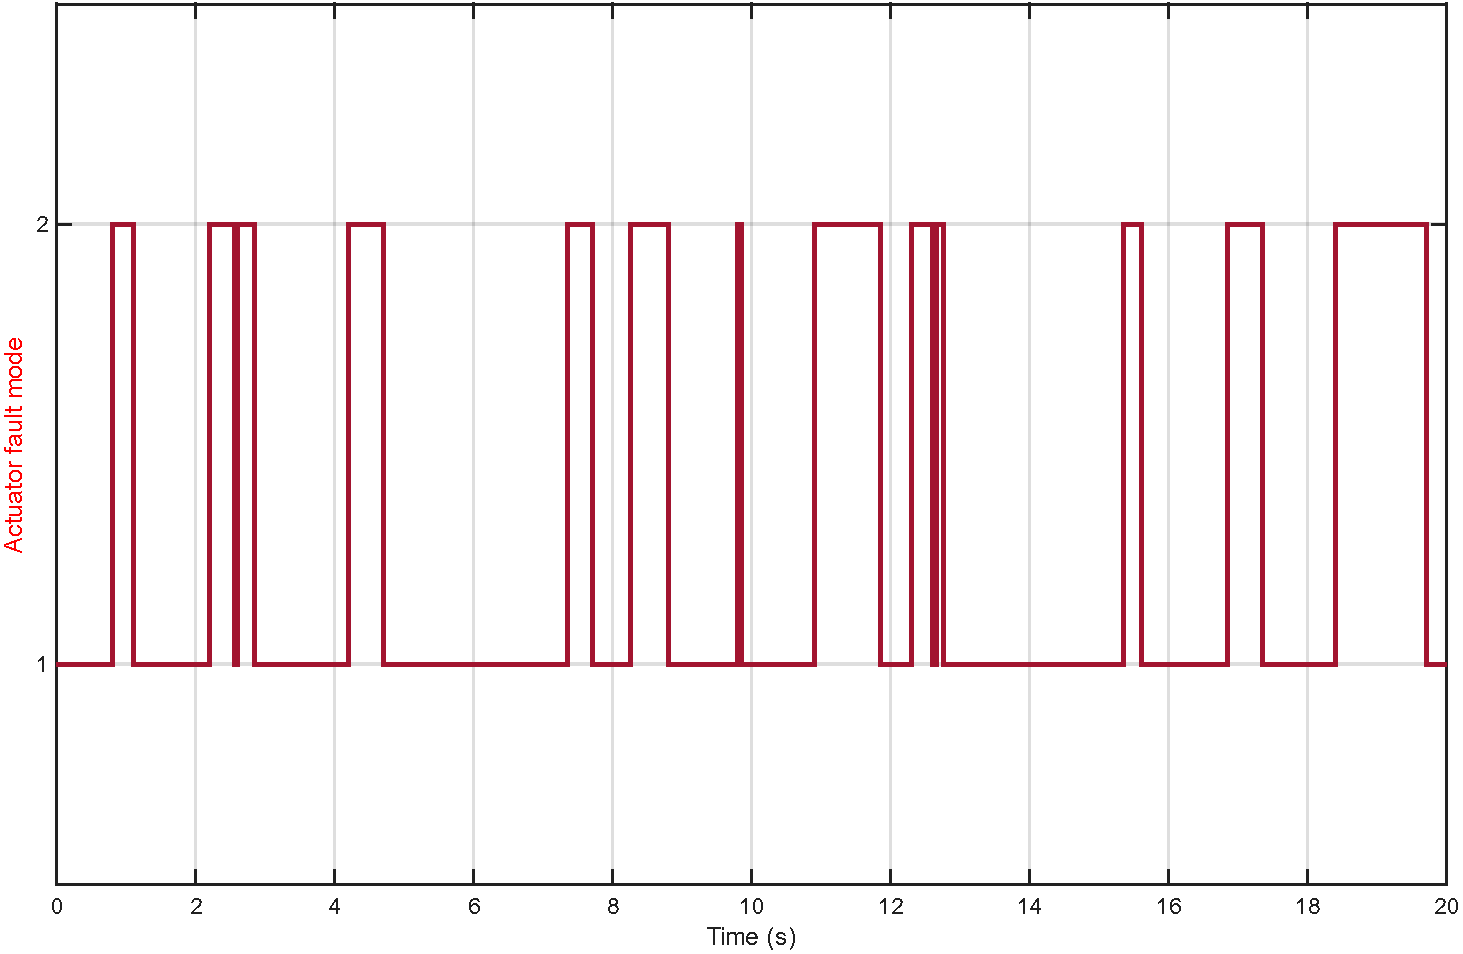
\includegraphics[width=\linewidth]{figs/actuator_fault.pdf}\par
  \smallskip
  {\small \textbf{Fig.~7.} Evolution of the actuator fault mode $r(t)$.\par}
\end{minipage}\par
\addvspace{\baselineskip}
\noindent\begin{minipage}{\linewidth}
  \centering
  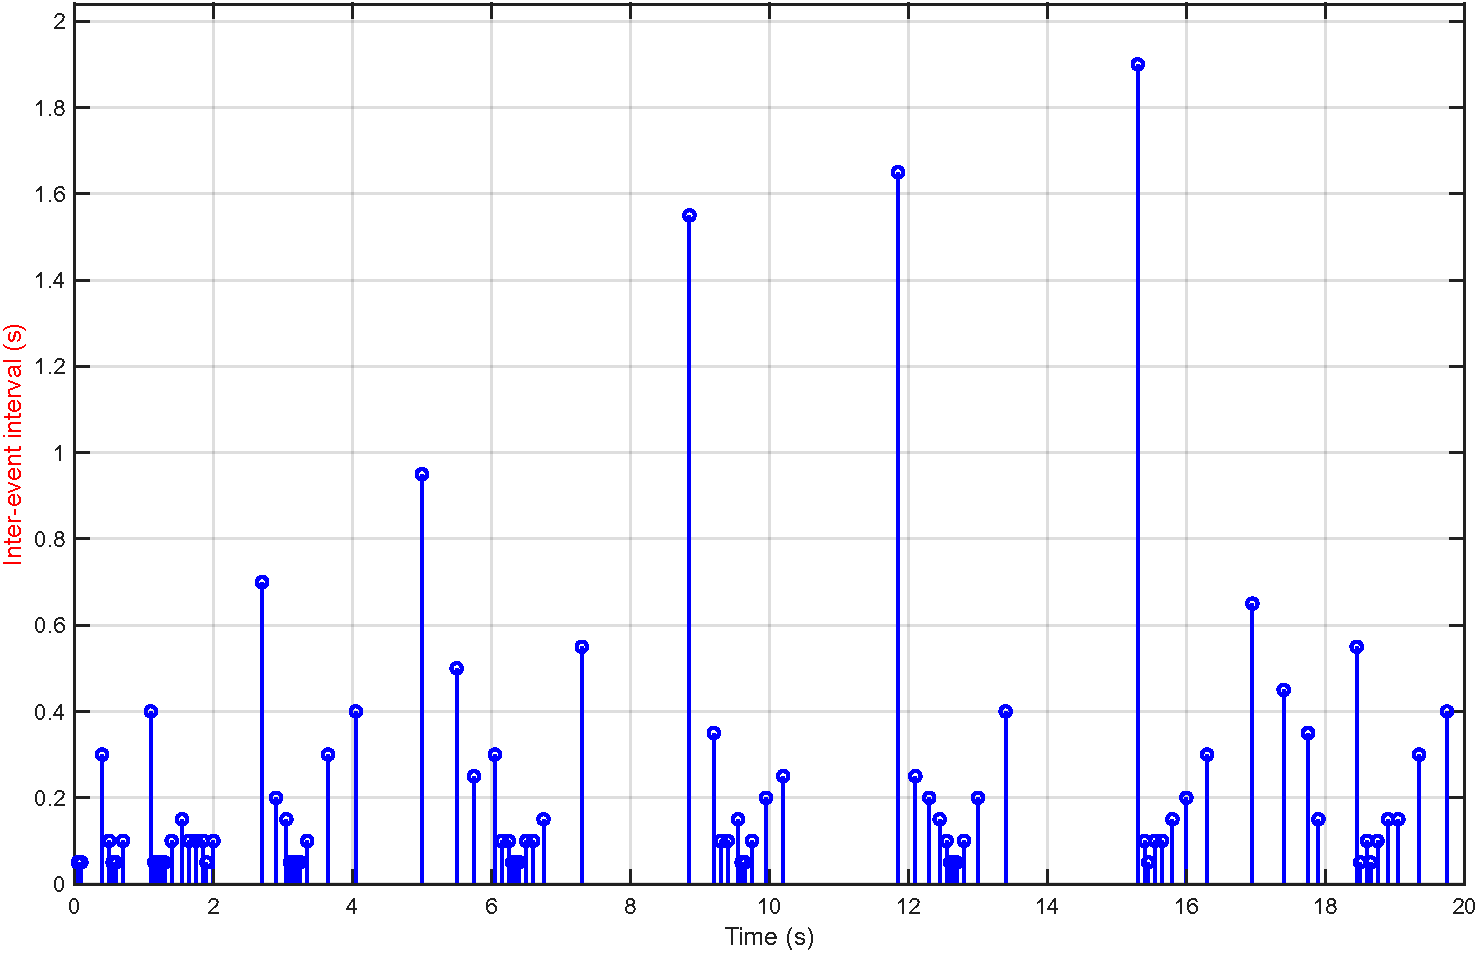
\includegraphics[width=\linewidth]{figs/event_tri_time.pdf}\par
  \smallskip
  {\small \textbf{Fig.~9.} Release instants and release intervals.\par}
\end{minipage}\par

% Previous type-1 reduction question and draft (absent from current reviews).
% Thank you for this insightful question. When the lower and upper membership functions coincide, the corresponding lower and upper firing strengths become identical. Since their weighting coefficients sum to one, the blended membership weight reduces to their common value under the normalization assumed in the model. Thus, the interval uncertainty disappears, and the model reduces to the type-1 fuzzy case. However, the resulting membership functions may still vary with the system state, and their derivatives need not be zero. Therefore, the derivative-sign-based regional partition, regional controller gains, and associated matrix constraints remain applicable. These features exploit membership variation rather than interval uncertainty itself. Accordingly, the existing stability and controller-synthesis conditions can be specialized to this type-1 case by substituting the corresponding membership functions, provided that the stated assumptions and LMI feasibility conditions remain satisfied.
%
%
% \textbf{Manuscript reference.} Section 2.1, Eqs. (2)–(4), and Section 2.4, Lemma 2.1 and Remark 2.4.

\end{document}
